% Adjust these for the path of the theme and its graphics, relative to this file
%\usepackage{beamerthemeFalmouthGamesAcademy}
	\usepackage{../../beamerthemeFalmouthGamesAcademy}
\usepackage{multimedia}
\graphicspath{ {../../} }

% Default language for code listings
\lstset{language=Python,
	morekeywords={each,in,nullptr,Bitmap,SetPixel,Color,Save,FromArgb, double, Math, Sqrt,public,static,string}
}

% For strikethrough effect
\usepackage[normalem]{ulem}
\usepackage{wasysym}

\usepackage{pdfpages}

% http://www.texample.net/tikz/examples/state-machine/
\usetikzlibrary{arrows,automata}

\title{\sessionnumber: Tinkering Graphics II}
\subtitle{\modulecode: \moduletitle}
\author{Michael Scott and Matt Watkins}

\setbeamertemplate{navigation symbols}{}

\newcommand{\fullbleed}[1]{
\begin{frame}[plain]
	\begin{tikzpicture}[remember picture, overlay]
		\node[at=(current page.center)] {
			\includegraphics[width=\paperwidth]{#1}
		};
	\end{tikzpicture}
\end{frame}
}

\newcommand{\picturepage}[2]{
\begin{frame}[plain]
	\begin{tikzpicture}[remember picture, overlay]
		\node[at=(current page.center)] {
			\includegraphics[width=\paperwidth]{#1}
		};
		\draw<1>[draw=none, fill=black, opacity=0.9] (-1,-5.2) rectangle (current page.south east);
		\node[draw=none,text width=0.96\paperwidth, align=right] at (5.5,-5.5) {\tiny{#2}};
	\end{tikzpicture}
\end{frame}
}

\newcommand{\notepicx}[5]{
\begin{frame}[plain]
	\begin{tikzpicture}[remember picture, overlay]
		\node[at=(current page.center)] {
			\includegraphics[width=\paperwidth]{#1}
		};
		\node[draw=none, fill=black, text width=#5\paperwidth] at ([xshift=#3, yshift=#4] current page.center) {\small{#2}};
	\end{tikzpicture}
\end{frame}
}

\newcommand{\notepic}[4]{
	\notepicx{#1}{#2}{#3}{#4}{0.4}
}
{\tiny }
\begin{document}

\maketitle

\begin{frame}
	\frametitle{Learning Outcomes}
	\begin{itemize}
		\item \textbf{Explain how} conditional logic can manipulate the output of a computer program
		\item \textbf{Apply} mathematical knowledge to \textbf{write} computer programs that manipulate pixels in a surface
		\item \textbf{Trace} existing computer programs
	\end{itemize}
\end{frame}

\begin{frame}
	\frametitle{House Keeping}
	
	This week we are going to focus on workflow. Less hacky more professional:
	
	\begin{itemize}		
		\item Make sure in your pair you have a shared repo on \textbf{Bitbucket}
		\item We will try to focus on portable code that uses \textbf{constants} over \textbf{literals}
		\item Reuse \textbf{functions} to build an effective code base.
		\item Link your functions to the Forms \textbf{UI} components
	
	\end{itemize}
\end{frame}

\begin{frame}[fragile]
	\frametitle{Recap - Functions in C\#}
	
	\begin{lstlisting}
public static string NameAndScore(string Name, int Score) 
{
	return "Name: " + Name + " Score: " + Score;
}		
string output = NameAndScore("Matt", 2345);		

	\end{lstlisting}
Variable 'output' is set to:
	\begin{lstlisting}
Name: Matt Score: 2345		

\end{lstlisting}
	
\end{frame}

\begin{frame}
	\frametitle{Distance Between Colors}
	
	Sometimes we need to measure when something is `close enough':
	
	\begin{itemize}		
		\item Distance between two points in the Cartesian coordinate system:
		\item $\sqrt{(x_{1} - x_{2})^2 + (y_{1} - y_{2})^2}$
		\item Distance between two colours in the RGB colour representation system:
		\item $\sqrt{(red_{1} - red_{2})^2 + (green_{1} - green_{2})^2 + (blue_{1} - blue_{2})^2}$
	\end{itemize}
\end{frame}

\fullbleed{distance-points}
\fullbleed{distance-colour}

\begin{frame}
	\frametitle{Activity \#1: Color Distance}
	
	In pairs:
	
	\vspace{2em}
	
	\begin{itemize}		
		\item Setup a basic project in Visual Studio
		\item Use the distance equation from the previous slide to write a function which accepts a two colours and returns the distance
		\item Test your solution
		\item Then, post your solution on Slack
	\end{itemize}
\end{frame}

\begin{frame}[fragile]
	\frametitle{Numeric Return Values}
	
\begin{lstlisting}
public static int GetDistance(Color first, Color second)
{
	int redDifference;
	int greenDifference;
	int blueDifference;
	double sqrt;

	redDifference = first.R - second.R;
	greenDifference = first.G - second.G;
	blueDifference = first.B - second.B;
	sqrt = Math.Sqrt(redDifference * redDifference + 
	greenDifference *  greenDifference +
	blueDifference * blueDifference);

	return sqrt;		
}
\end{lstlisting}


\end{frame}

\begin{frame}[fragile]
	\frametitle{Expected Output: Color Distance}
 You can use predefined color names with this method:
\begin{lstlisting}
Color Color1 = Color.FromKnownColor(KnownColor.Pink);	
\end{lstlisting}
Expected Values:	
\begin{lstlisting}
Console.WriteLine (GetDistance(WHITE, BLACK));
- 195075
Console.WriteLine (GetDistance(WHITE, PINK));
- 6673
Console.WriteLine (GetDistance(BLACK, PINK));
- 143098
Console.WriteLine (GetDistance(MAGENTA DARKGOLDENROD));
- 82533
\end{lstlisting}
NOTE - You need to create the color objects and pass them into the function, don't just use a colour in capitals. just for illustration.  
\end{frame}

\begin{frame}
	\frametitle{Activity \#2: Colour Tolerance}
	
	In pairs:
	
	\vspace{.5em}
	
	\begin{itemize}		
		\item Setup a Windows forms project in Visual Studio
		\item Implement the function \texttt{closeEnough((colour1, colour2), tolerance)} that returns a boolean value
		\item Test your solution
		\item Then, post your solution on Slack
	\end{itemize}
	\vspace{.5em}
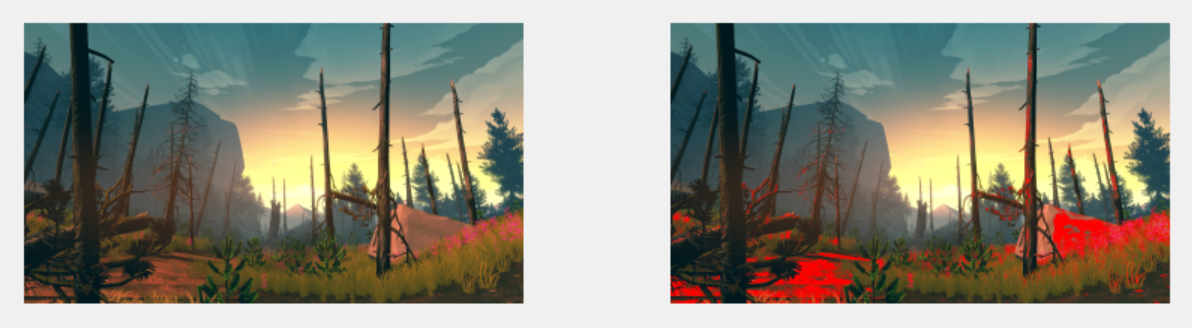
\includegraphics[scale=0.5]{GoingRed}
\end{frame}

\begin{frame}[fragile]
	\frametitle{Boolean Return Values}
	
\begin{lstlisting}
public static bool closeEnough(Color first, Color second) {
	int redDifference;
	int greenDifference;
	int blueDifference;
	redDifference = first.R - second.R;
	greenDifference = first.G - second.G;
	blueDifference = first.B - second.B;
	
	if ((redDifference * redDifference + greenDifference
	* greenDifference + blueDifference * blueDifference)
	< 300)	{
		return true;
	} else {
		return false;
	}
}
\end{lstlisting}

Note: This source code should be used in conjunction with a function call to activate it.

\end{frame}

\begin{frame}[fragile]
	\frametitle{Tolerance-based Pixel Manipulation}
	
\begin{lstlisting}
public static bool turnRed(Color newColour) {
	Color brown = Color.FromKnownColor(KnownColor.Brown);
	int redDifference;
	int greenDifference;
	int blueDifference;
	redDifference = newColour.R - brown.R;
	greenDifference = newColour.G - brown.G;
	blueDifference = newColour.B - brown.B;
	
	if ((redDifference * redDifference + greenDifference
	* greenDifference + blueDifference * blueDifference)
	 < 4000) {
		return true;
	} else {
		return false;
	}	
}

\end{lstlisting}


\end{frame}

\begin{frame}[fragile]
	\frametitle{Tolerance-based Pixel Manipulation}
	
	\begin{lstlisting}
Color p;

for (int y = 0; y < height; y++) {
	for (int x = 0; x < width; x++) {
		p = bmp.GetPixel(x, y);
		if (turnRed(p))	{
			bmp.SetPixel(x, y, Color.FromKnownColor
			(KnownColor.Red));
		}
	}
}
		
	\end{lstlisting}
Note: This uses the function from the previous screen. To achieve the outcome that you want you may need to tinker with the tolerance level to quite a high number.	
	
\end{frame}
		

\begin{frame}
	\frametitle{Red Eye}
	
	\begin{itemize}		
		\item When the flash of the camera catches the eye just right (especially with light colored eyes), we get bounce back from the back of the retina.
		\item This results in `red eye'
		\item We can replace the “red” with a color of our choosing
		\item First, we figure out where the eyes are (x,y)
	\end{itemize}
\end{frame}

\fullbleed{jenny}

\begin{frame}[fragile]
	\frametitle{Activity \#3: Red Eye}
	
	In pairs:
	
	\vspace{1em}
	
	\begin{itemize}		
		\item Setup a Windows form project in Visual Studio
		\item You will need to create a method to sample a specific area of the image. I suggest you sample the mouse position.
		\end{itemize}
	\begin{lstlisting}
private void pictureBox1_MouseUp(object sender,
MouseEventArgs e)
{
	mouseX = e.X;
	mouseY = e.Y;
}
\end{lstlisting}
	\begin{itemize}	
		\item Implement the function: \texttt{removeRedEye(picture, area, colour)}
		\item Test your solution
		\item Then, post your solution on Teams
	\end{itemize}


\end{frame}

\fullbleed{sample_area}
\fullbleed{jenny_nored}

\begin{frame}
	\frametitle{Posterization}
	
	\begin{itemize}			
		\item Posterization is simply reducing the number of colours in an image
		\item We look for a range of colours, then map them to a single colour, e.g:
		\begin{itemize}
			\item If red is between 63 and 128, set it to 95
			\item If green is less than 64, set it to 31
		\end{itemize}	
		\item The end result is that a bunch of different colours, get set to a few colours
		\item Beware of naive solutions with a large number of `if' statements
	\end{itemize}
\end{frame}

\fullbleed{ben}

\begin{frame}
	\frametitle{Calculating Luminance in RGB}
	
	To do this, we may need to determine the luminance of a pixel:
	
	\begin{itemize}		
		\item Luminance is the overall brightness of a pixel
		\item In RGB, it is the \textit{mean} average value of each component:
		\begin{itemize}
			\item $lum = (red + green + blue) / 3$
		\end{itemize}	
	\end{itemize}
\end{frame}



\begin{frame}
	\frametitle{Activity \#5: Black and White}
	
	In pairs:
	
	\vspace{2em}
	
	\begin{itemize}		
		\item Setup a Windows form project in Visual Studio
		\item Refer to the following documentation
		\item Implement the function: \texttt{makeGreyscale(picture, colourCount)}
		\item Test your solution
		\item Then, post your solution on Slack
	\end{itemize}
\end{frame}

\begin{frame}[fragile]
	\frametitle{Source Code: Black and White}
	
\begin{lstlisting}
for (int y = 0; y < height; y++) {
	for (int x = 0; x < width; x++)	{
		p = bmp.GetPixel(x, y);
		int r = p.R;
		int g = p.G;
		int b = p.B;
		int luminance = (r + g + b) / 3;
		// start at 64 to see the difference
		if (luminance < 104)	{
			bmp.SetPixel(x, y, Color.FromArgb(255, 0, 0,
			 0));
		}
		if (luminance >= 104)	{
		 	bmp.SetPixel(x, y, Color.FromArgb(255, 255, 
		 	255, 255));
		}
	}
}
\end{lstlisting}



\end{frame}

\begin{frame}
	\frametitle{Sepia Tone}
	
	\begin{itemize}		
		\item Pictures that are sepia-toned have a yellowish tint to them that we associate with older pictures.
		\item It's not directly a matter of simply increasing the yellow in the picture, because it's not a one-to-one correspondence:
		\begin{itemize}
			\item Instead, colors in different ranges get mapped to other colours.
			\item We can create such a mapping using IF statements
		\end{itemize}	
		\item The end result is that a bunch of different colours, get set to a few colours
		\item Beware of naive solutions with a large number of `if' statements
	\end{itemize}
\end{frame}

\fullbleed{field_normal}

\fullbleed{field_sepia}

\begin{frame}
	\frametitle{Sepia Tone}
	
	\begin{itemize}		
		\item First, we're calling greyScaleNew (the one with weights).
		\item We then manipulate the red (increasing) and the blue (decreasing) channels to bring out more yellows and oranges.
		\begin{itemize}
			\item It's perfectly okay to have one function calling another.
			\item Why are we doing the comparisons on the red? Why not?  After greyscale conversion, all channels are the same!
		\end{itemize}	
		\item The end result is that a bunch of different colours, get set to a few colours
		\item Why these values? Trial-and-error: Tinker the values!

	\end{itemize}
\end{frame}

\begin{frame}[fragile]
	\frametitle{Source Code: Sepia (1)}
	
\begin{lstlisting}
public void sepiaTint(picture) {
	//Convert image to greyscale
  	makeGreyscale(picture);  
	for (int y = 0; y < height; y++)
	{
		for (int x = 0; x < width; x++)
		{
			p = picture.GetPixel(x, y);
			
			int r = p.R;
			int g = p.G;
			int b = p.B;

			if (r < 63)
			{
				r = r*1.1;
				b = b*0.9;
			}			
...
\end{lstlisting}

\end{frame}

\begin{frame}[fragile]
	\frametitle{Source Code: Sepia (2)}
	
\begin{lstlisting}
...
			if (r > 62 and r < 192) {
				bmp.SetPixel(x, y, Color.FromArgb(
				255, 255, 255, 255));
			}
			if (r > 191) {
				r = r*1.08;
				if (r > 255) {
					r = 255; 	
				}
				b = b*0.93;
			}

		}
	}	
}

\end{lstlisting}
Note: This requires that you incorporate a greyscale function as well.

\end{frame}

\begin{frame}
	\frametitle{Activity \#6: Sepia Tone}
	
	In pairs:
	
	\vspace{2em}
	
	\begin{itemize}		
		\item Setup a Windows form project in Visual Studio
		\item Refer to the following documentation
		\item Refactor the function: \texttt{sepiaTint(picture) to use constants rather than literals}
		\item Tinker with the values of the constants to test your solution
		\item Then, post your solution on Slack
	\end{itemize}
\end{frame}

\end{document}
